Database search identified 1367 publications, of which \x{n.all} studies met the inclusion criteria
(Figure~\ref{fig:prisma}).
Several models of \hiv progression and treatment were excluded as they did not model \hiv transmission,
and several models simulating vertical transmission were excluded as they were not dynamical.
Table~\ref{tab:summary} summarizes the basic characteristics of the models in each study.
%The complete data extraction spreadsheet is available online.%
%\footnote{\hreftt{https://docs.google.com/spreadsheets/d/1GI2g1Kg7xOFRrEpXLwJUHySkcgLrdBMt-56qwLG3ylA}}
\begin{figure}[h]
  \centering
  \newcommand{\nprisma}[2]{\textbf{#2} (N~{=}~#1)}%
\newcommand{\nprismasub}[2]{\parbox{4ex}{\hfill#1}: #2\\}%
\begin{tikzpicture}[xscale=5.5,yscale=1.8]
  \scriptsize
  % boxes
  \node[prisma](a0) at (0, 0.0) {\nprisma{2134}{Database search hits\\}};
  \node[prisma](a1) at (1, 0.0) {\nprisma {767}{Duplicates removed automatically\\}};
  \node[prisma](b0) at (0,-1.0) {\nprisma{1367}{Abstracts screened\\}};
  \node[prisma](b1) at (1,-1.0) {\nprisma {595}{Irrelevant\\}};
  \node[prisma](c0) at (0,-2.0) {\nprisma {772}{Full texts assessed\\}};
  \node[prisma](c1) at (1,-2.0) {\nprisma {424}{Excluded}\\\raggedright
    \nprismasub{  4}{Duplicate}
    \nprismasub{115}{Publication type}
    \nprismasub{118}{No transmission modelling}
    \nprismasub{136}{Not dynamical model}
    \nprismasub{ 12}{Not SSA}
    \nprismasub{ 25}{Not HIV}
    \nprismasub{ 17}{Model comparison}};
  \node[prisma](d0) at (0,-3.7) {\nprisma{360}{Dynamical HIV transmission model\\}};
  \node[prisma](d1) at (1,-3.7) {\nprisma{266}{Excluded}\\\raggedright
    \nprismasub{105}{Individual-based model}
    \nprismasub{161}{No ART scale-up scenario}};
  \node[prisma](e0) at (0,-4.7) {\nprisma{94}{Any ART scale-up scenario\\}\\\textit{Dataset~A}};
  \node[prisma](e1) at (1,-4.7) {\nprisma{54}{Excluded}\\\raggedright
    \nprismasub{23}{Only combination interventions}
    \nprismasub{14}{Reported other measures}
    \nprismasub{ 8}{No status quo base case scenario}
    \nprismasub{ 4}{Only ART targeted to risk groups}
    \nprismasub{ 1}{Repeated modelling analysis}};
  \node[prisma](f0) at (0,-5.7) {\nprisma{40}{Infections averted / incidence reduction due to ART scale-up for all\\}\\\textit{Dataset~B}};
  % arroes
  \draw[arrow] (a0) -- (a1);
  \draw[arrow] (a0) -- (b0);
  \draw[arrow] (b0) -- (b1);
  \draw[arrow] (b0) -- (c0);
  \draw[arrow] (c0.east) -- (c1.west|-c0.east);
  \draw[arrow] (c0) -- node[right]{$+$12 Cited Studies} (d0);
  \draw[arrow] (d0.east) -- (d1.west|-d0.east);
  \draw[arrow] (d0) -- (e0);
  \draw[arrow] (e0.east) -- (e1.west|-e0.east);
  \draw[arrow] (e0) -- (f0);
\end{tikzpicture}

  \caption{\textsc{prisma} flowchart of study identification [numbers not final]}
  \label{fig:prisma}
\end{figure}
\begin{table}
  \centering
  \caption{Basic characteristics of transmission models used}
  \searchsize
\begin{tabular}{R{.02}R{.07}L{.82}}
	\toprule
	  &          Term & Hits                 \\
	\midrule
	1 & \num{1369153} & \st{[model]}         \\
	2 &  \num{954470} & \st{[hiv]}           \\
	3 &  \num{982505} & \st{[ssa]}           \\
	4 &    \num{2190} & \st{1 AND 2 AND 3}   \\
	5 &    \num{1384} & \st{4 NOT [exclude]} \\
	\bottomrule
\end{tabular}
  \label{tab:summary}
\end{table}
% ==============================================================================
\subsection{Context \& Applications}
\label{ss:res:app}
Most studies simulated \hiv transmission at the national level,
including \x{n.geo.national} single-country and \x{n.geo.national.multi} multi-country analyses.
Studies also explored
super-national~(\x{n.geo.ssa}),
sub-national~(\x{n.geo.any.sub.national}), and
city-level~(\x{n.geo.any.city}) epidemic scales.
South Africa was the most common context simulated
(\x{n.South-Africa} studies, Figure~\ref{fig:map}),
but was not disproportionately represented among \ssa countries, since
the number of transmission modelling studies per million \plhiv as of 2019
in South Africa (\x{mph.South-Africa})
was not above the \ssa median (\x{mph.med}).
Kenya was the next most common with \x{n.Kenya} modelling studies.
\begin{figure}[h]
  \centering
  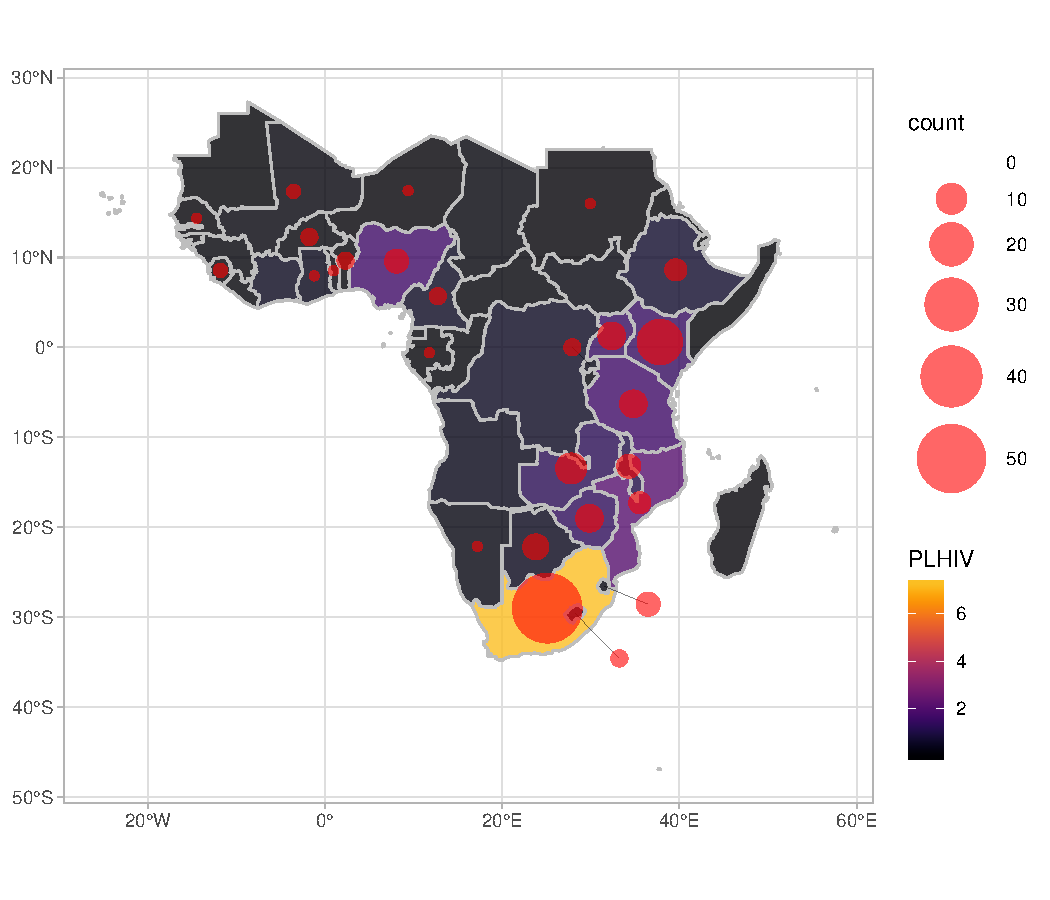
\includegraphics[width=0.8\linewidth]{map-n-vs-plhiv}
  \caption{Number of dynamical \hiv transmission modelling studies per country (circle area)
    vs million \plhiv (fill) as of 2019 from \cite{AIDSinfo}.}
  \label{fig:map}
\end{figure}
% ==============================================================================
\subsection{Interventions}
\label{ss:res:int}
\begin{figure}
  \centering
  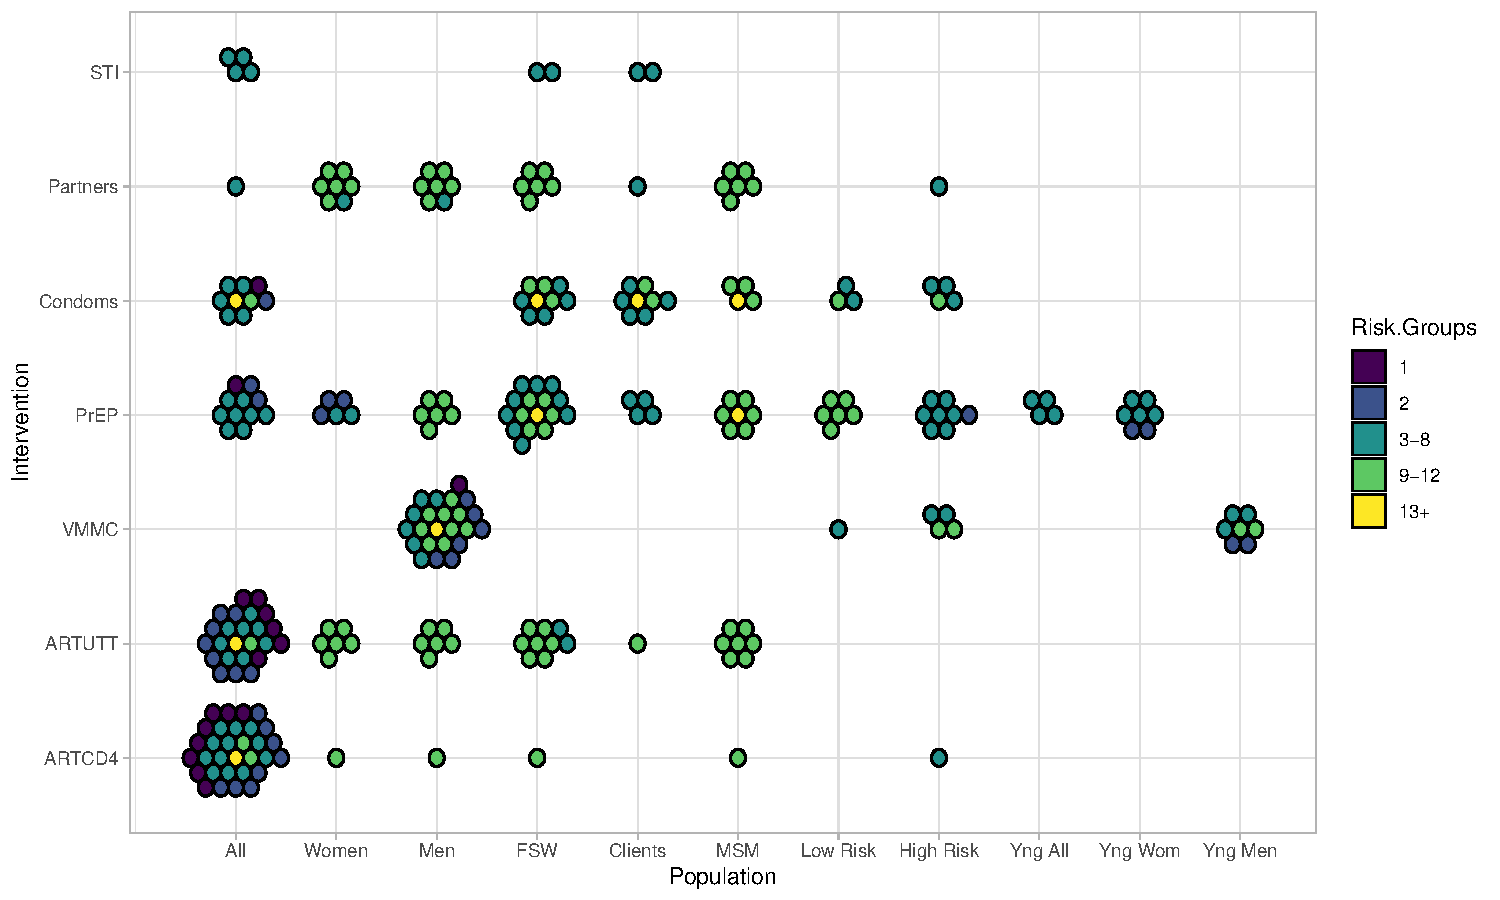
\includegraphics[width=0.9\linewidth]{ints-vs-pops}
  \caption{Number of studies simulating counterfactual interventions
    prioritizing specific risk groups (points),
    and the total number of risk groups in each model (fill colour).}
  \floatfoot{%
    Studies may appear more than once if
    multiple prioritized populations and/or interventions were simulated.}
  \label{fig:ints-vs-pops}
\end{figure}
The population-level prevention benefits of increased \art coverage
was simulated in \x{n.RQi.ART.any} studies, including
\x{n.RQi.ARTCD4} studies examining increased coverage under \cdf thresholds, and
\x{n.RQi.ARTUTT} studies examining \utt
(\x{n.RQi.ART.both} studies examined both).
Increasing \art coverage under any eligibility criteria
was rarely prioritized to any risk group
(only \x{n.RQi.ART.pri} of \x{n.RQi.ART.any} studies),
although several studies by \textcite{Anderson2014}
explored prioritization of \art to women, men, \fsw, and \msm under \utt
(Figure~\ref{fig:ints-vs-pops}).
Before 2015 (\who began recommending \utt),
\x{n.RQi.ARTCD4.all} and \x{n.RQi.ARTUTT.all} studies examined
non-prioritized scale-up of \art under \cdf thresholds and \utt respectively,
while only \x{n.RQi.ARTCD4.pri} and \x{n.RQi.ARTUTT.pri} examined prioritized scale-up.
\par
Most studies examining \vmmc interventions did not explore prioritization
to risk groups among men.
By contrast, counterfactual \prep interventions
were prioritized to a wide range of risk groups, especially \fsw.
Among simulated behavioural interventions,
condom promotion was often prioritized to sex work,
whereas decreasing partnership formation rates was simulated among
women, men, \fsw, and \msm mostly by \textcite{Anderson2014}.
The most commonly simulated historical interventions were increasing
\art coverage (\x{n.BHi.ART}),
condom use (\x{n.BHi.Condoms}), and
\vmmc (\x{n.BHi.VMMC}), followed by
a generic reduction in force of infection (\x{n.BHi.Generic}), according either to
\hiv prevalence as in \cite{Williams2006},
or calendar time as in \cite{Awad2015a}.
The inclusion of any historical intervention increased with publication year
($p = \x{BHi-vs-pub.year-p}$).
\par
Regarding intervention combinations,
Figure~\ref{fig:cooc} illustrates the number of studies simulating:
(\subref{fig:cooc-hh}) combinations of multiple historical interventions;
(\subref{fig:cooc-hn}) combinations of counterfactual interventions and historical interventions; and
(\subref{fig:cooc-nn}) combinations of counterfactual interventions.
Additional \art scale-up, \vmmc, and \prep interventions were often simulated against
historical increases in \vmmc, condom use, and especially \art scale-up.
By contrast, behavioural interventions (increasing condom use \& decreasing partners)
were less likely to be simulated against historical interventions.
Counterfactual combination interventions most often included
\art (especially \utt), \vmmc, and \prep.
Table~\ref{tab:combo} summarizes the complete selection of particular combinations explored.
\begin{figure}
  \centering
  \begin{subfigure}{0.33\linewidth}
    \centering
    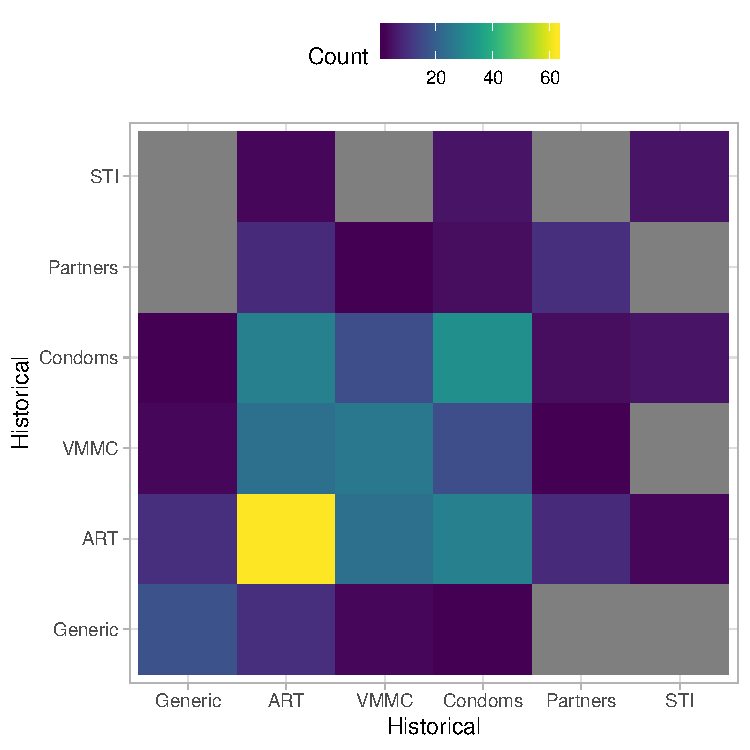
\includegraphics[width=\linewidth]{ints-cooc-h-vs-h}
    \caption{Historical combinations}
    \label{fig:cooc-hh}
  \end{subfigure}%
  \begin{subfigure}{0.33\linewidth}
    \centering
    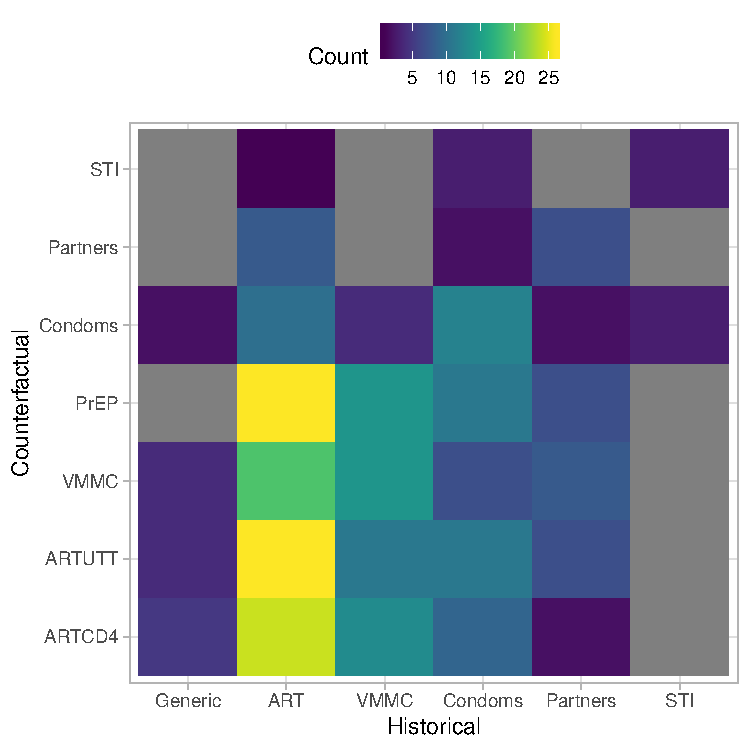
\includegraphics[width=\linewidth]{ints-cooc-h-vs-n}
    \caption{Counterfactual with historical}
    \label{fig:cooc-hn}
  \end{subfigure}%
  \begin{subfigure}{0.33\linewidth} % TODO: kill?
    \centering
    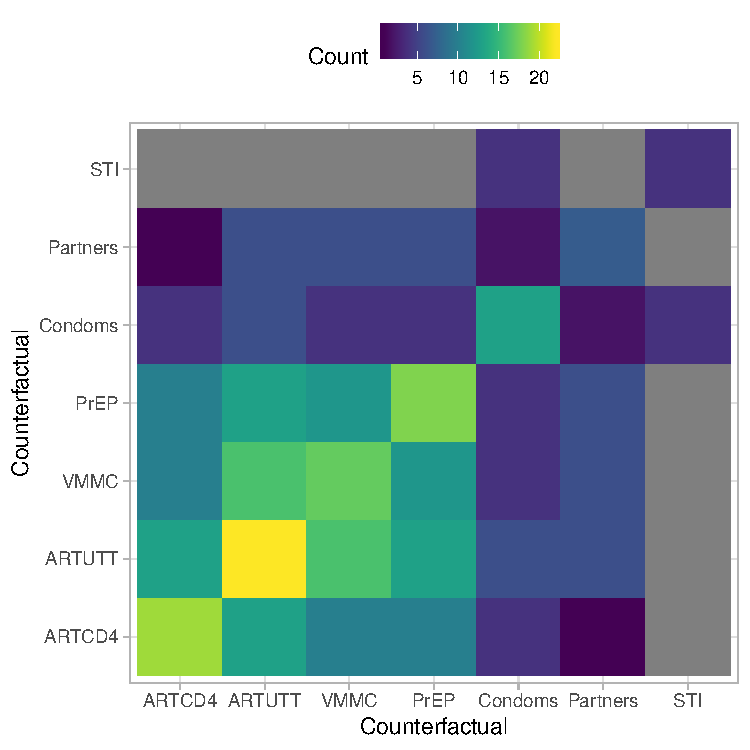
\includegraphics[width=\linewidth]{ints-cooc-n-vs-n}
    \caption{Counterfactual combinations}
    \label{fig:cooc-nn}
  \end{subfigure}%
  \caption{Co-occurrence of modelled historical and counterfactual interventions}
  \floatfoot{%
    Historical: simulated to reflect existing interventions;
    Counterfactual: hypothetical interventions whose impact is being evaluated;
    See \ref{ss:meth:data} for additional definitions.}
%  could be twice.
  \label{fig:cooc}
\end{figure}
\begin{table}
  \centering
  \caption{Counterfactual combination interventions simulated}
  \newcommand{\Y}{\textbullet}
\begin{tabular}{cccccc}
	\toprule
	       \multicolumn{5}{c}{Intervention}        &                                                      \\
	\cmidrule(rl){1-5}
	  \art    & \vmmc & \prep & Condoms &  Other   & Studies                                              \\
	\midrule
	\cdf/\utt & \vmmc &       &         &          & \x{n.combo.ARTCD4.ARTUTT.VMMC}                       \\
	\cdf/\utt & \vmmc & \prep &         &          & \x{n.combo.ARTCD4.ARTUTT.VMMC.PrEP}                  \\
	\cdf/\utt & \vmmc & \prep & Condoms &          & \x{n.combo.ARTCD4.ARTUTT.VMMC.PrEP.Condoms}          \\
	\cdf/\utt & \vmmc & \prep & Condoms & Partners & \x{n.combo.ARTCD4.ARTUTT.VMMC.PrEP.Condoms.Partners} \\
	\cdf/\utt &       & \prep &         &          & \x{n.combo.ARTCD4.ARTUTT.PrEP}                       \\
	\cdf/\utt &       &       &         & Generic  & \x{n.combo.ARTCD4.ARTUTT.Generic}                    \\
	  \cdf    &       & \prep &         &          & \x{n.combo.ARTCD4.PrEP}                              \\
	  \cdf    &       &       & Condoms &          & \x{n.combo.ARTCD4.Condoms}                           \\
	  \utt    & \vmmc & \prep &         & Partners & \x{n.combo.ARTUTT.VMMC.PrEP.Partners}                \\
	  \utt    & \vmmc &       & Condoms &          & \x{n.combo.ARTUTT.VMMC.Condoms}                      \\
	  \utt    &       & \prep & Condoms &          & \x{n.combo.ARTUTT.PrEP.Condoms}                      \\
	  \utt    &       &       & Condoms &          & \x{n.combo.ARTUTT.Condoms}                           \\
	          & \vmmc & \prep &         & Cash     & \x{n.combo.VMMC.PrEP.Cash}                           \\
	          &       & \prep & Condoms &          & \x{n.combo.PrEP.Condoms}                             \\
	          &       &       & Condoms & Partners & \x{n.combo.Condoms.Partners}                         \\
	          &       &       & Condoms &   \sti   & \x{n.combo.Condoms.STI}                              \\
	\bottomrule
\end{tabular}
  \label{tab:combo}
  \floatfoot{%
    See \ref{ss:meth:data} for intervention definitions.}
\end{table}
\subsection{Parameterizations of Risk Heterogeneity}
\label{ss:res:risk}
\paragraph{Risk Groups}
Among compartmental models,
the median (\iqr) number of risk groups modelled was \x{RG.n.q2}~(\x{RG.n.q1},~\x{RG.n.q3})
when considering sex as a risk stratification, and \x{RGz.n.q2}~(\x{RGz.n.q1},~\x{RGz.n.q3}) otherwise.
In univariate analysis, the number of risk groups increased significantly with
publication year ($p = \x{RG.n-vs-pub.year-p}$),
and in studies assessing counterfactual \vmmc and \prep interventions
($p = \x{RG.n-vs-VMMC-p}$ and $p = \x{RG.n-vs-PrEP-p}$, respectively).
Besides sex, risk groups were primarily defined by rates of partnership formation (\x{n.RG.np}),
followed by different types of partnerships formed (\x{n.RG.pt}).
Baseline turnover of individuals between at any risk groups was simulated in \x{n.RG.turnover} studies,
while an additional \x{n.RG.turn.bal} studies simulated turnover only to
maintain constant risk group proportions under differential \hiv-related mortality.
\par
Among \x{n.age.any} studies that stratified the population by age,
[TODO: mixing, explicit age risk].
\paragraph{Key Populations \& Partnership Types}
FSW were modelled in \x{n.KP.FSW} studies,
although \x{n.KP.FSW.semi} additional studies simulated
risk groups having similar relative rates of partnership formation
[TODO: update based on clearer definitions].
Sex work partnerships were explicitly modelled in \x{n.PT.SW} studies, defined by:
lower volumes of sex (XX), higher condom use (XX), or both (XX).
Casual partnerships were also modelled in \x{n.PT.casual} studies,
of which XX also modelled sex work;
casual partnerships were similarly defined by:
lower volumes of sex (XX), higher condom use (XX), or both (XX).
% In progress...
\begin{figure}
  \centering
  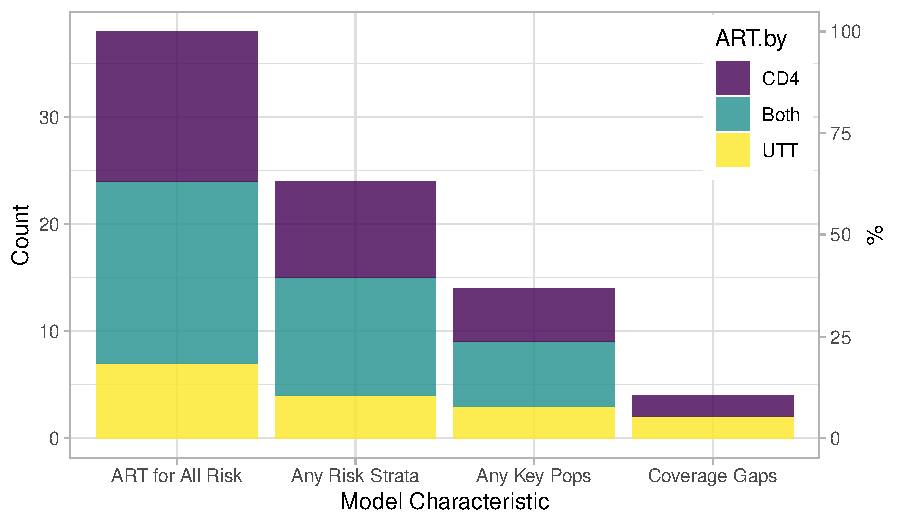
\includegraphics[width=0.7\linewidth]{risk-cascade}
  \caption{Model heterogeneity cascade among studies assessing
    counterfactual scale-up of ART equally across all modelled risk groups.
    Coverage gaps represents acknowledgement of differential (lower) coverage among key populations.}
\end{figure}


\par
The median (\iqr) number of \hiv infection states modelled was 3~(2,~4.5),
and 63\% of studies considered transient increased infectivity associated with acute infection.

